\appendix

\section{Visualization}

To better understand what the learned indexer selects, we visualize the per-head Index Branch selection probability over all query-block and key-block pairs in \Figref{fig:vis-selection}. We show four heads from an early layer (Layer~1) and a later layer (Layer~18), corresponding to four different GQA groups. Across layers, the learned sparse pattern recovers the main structures expected from dense attention: all heads place high probability on the local diagonal, consistently select the sink column, and reserve the remaining budget for a small number of long-range relative positions. At the same time, the non-local selections are not identical across GQA groups. Different groups attend to different long-range stripes while sharing the common local and sink patterns, suggesting that the learned indexer captures group-specific sparse attention patterns rather than collapsing to a single global selection pattern.

\begin{figure}[!htb]
\centering
\begin{subfigure}[t]{0.48\linewidth}
  \centering
  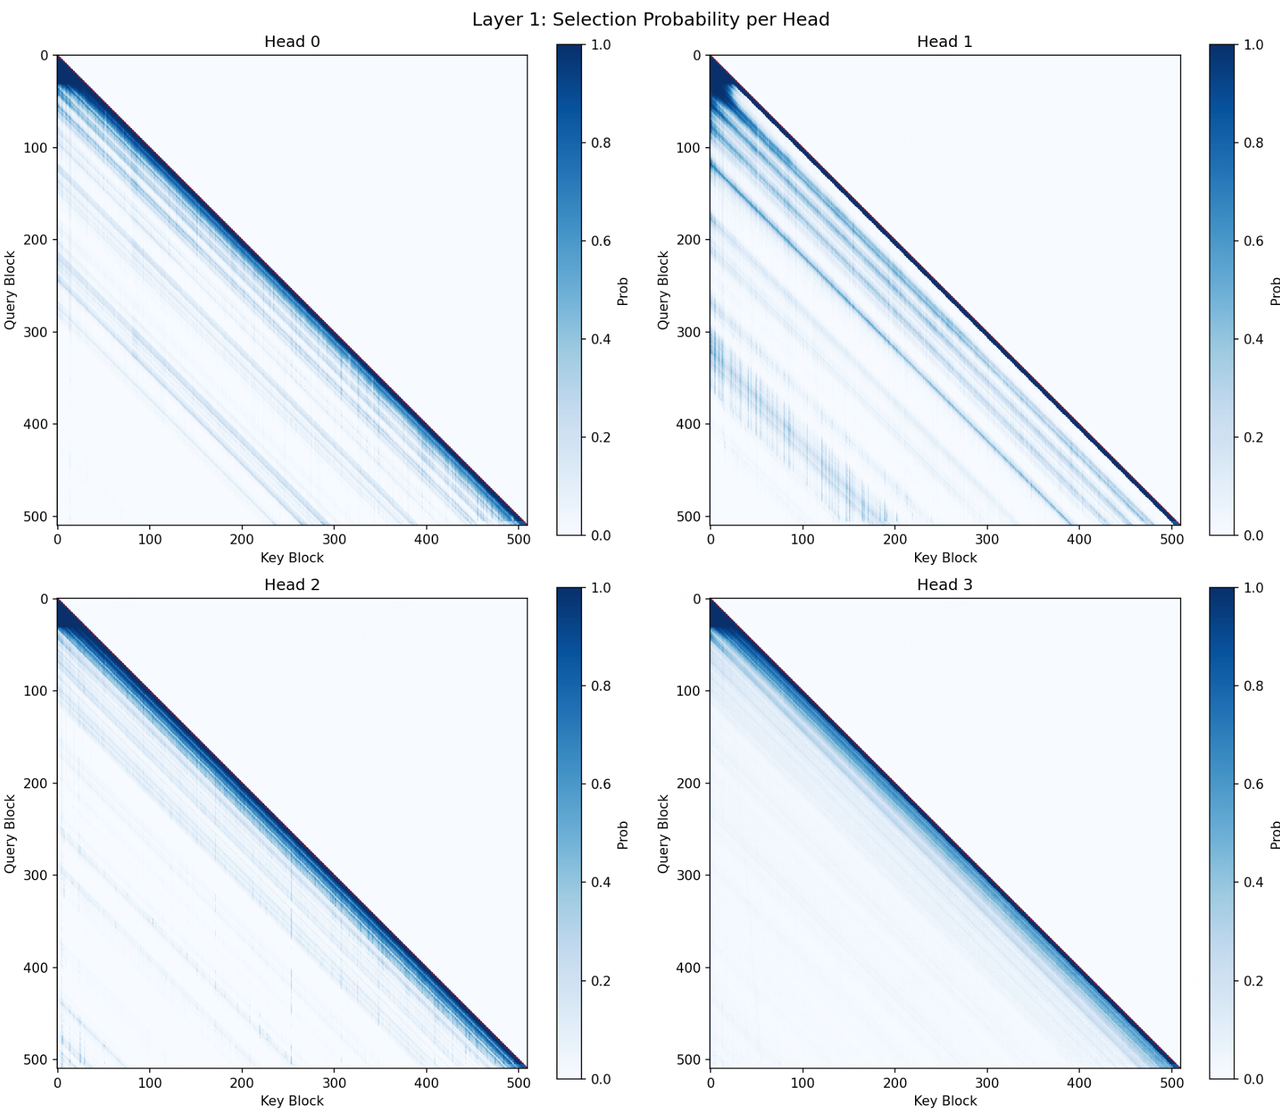
\includegraphics[width=\linewidth]{figures/vis_analysis_2.png}
  \caption{Layer 1, four GQA groups. Each group produces a different long-range selection pattern alongside the shared local diagonal and sink column.}
\end{subfigure}\hfill
\begin{subfigure}[t]{0.48\linewidth}
  \centering
  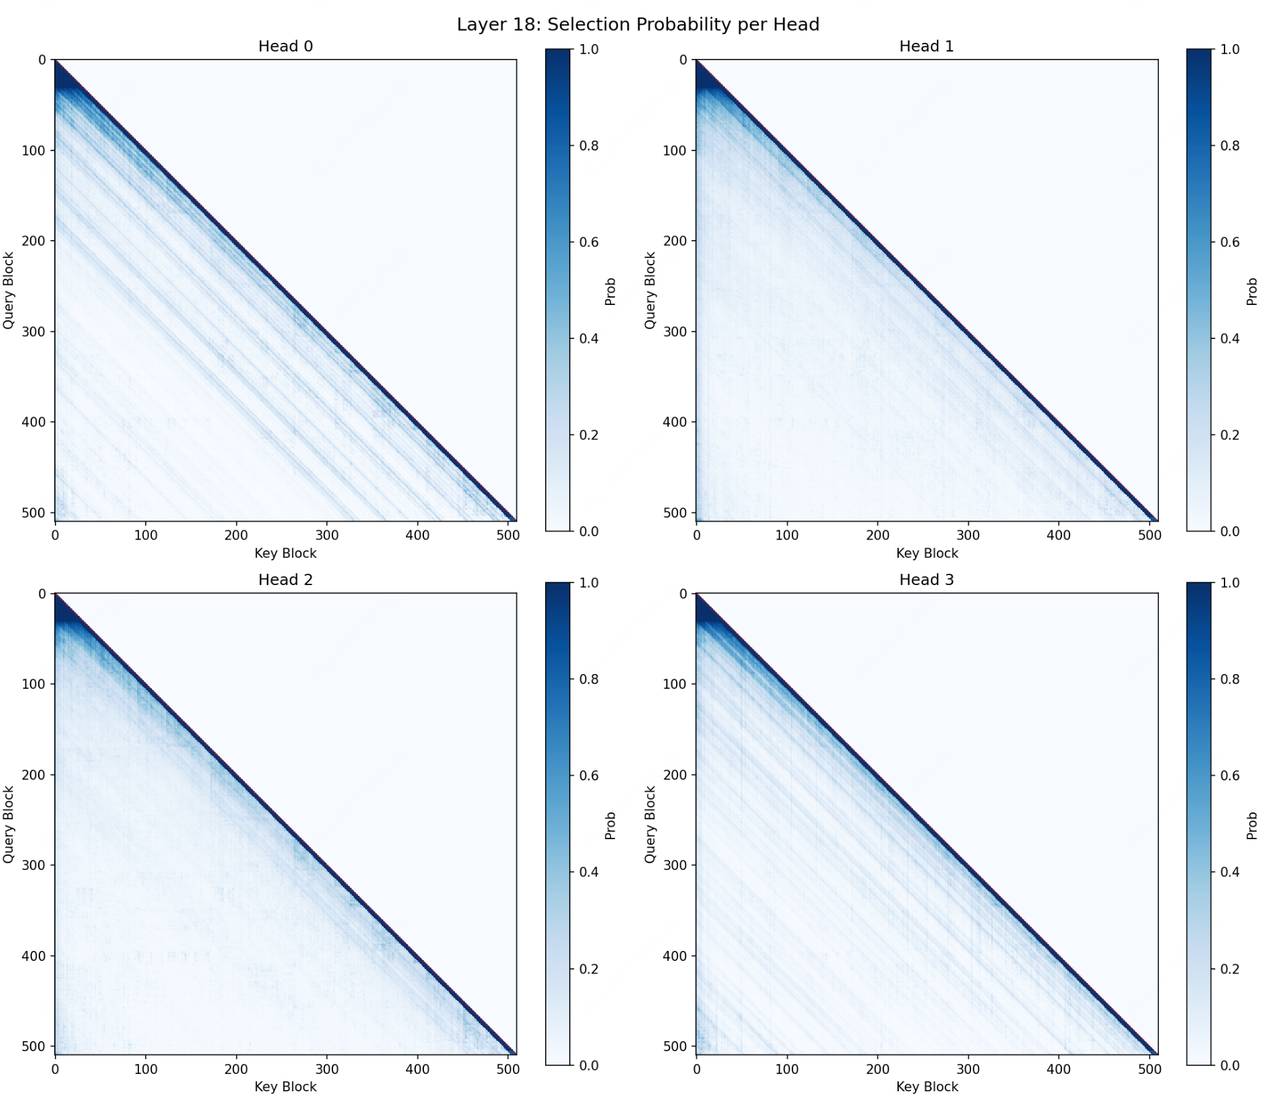
\includegraphics[width=\linewidth]{figures/vis_analysis_3.png}
  \caption{Layer 18, four GQA groups. Long-range selection sharpens into a few stripes per group; the four groups pick visibly different stripes.}
\end{subfigure}
\caption{Per-head Index Branch selection probability across query-key pairs. Each panel shows four heads from one layer, corresponding to four different GQA groups. All groups consistently select the local diagonal and the sink column (leftmost), while different groups trace different long-range stripes, revealing group-specific sparse selection patterns.}
\label{fig:vis-selection}
\end{figure}


We further examine the attention sink phenomenon in \method{} models. Even without explicitly forcing the indexer to select the first key-value block, we observe that the learned Index Branch naturally assigns high selection probability to the initial block across all layers and heads. \Figref{fig:attention-sink} shows results for two representative layers (Layer~4 and Layer~24), each with eight sampled heads. Across both layers, every head directs a substantial fraction of its attention mass to the first token. This confirms that attention focal points naturally emerge and are universally present across different heads and layers, even in our sparse attention mechanism.

\begin{figure}[!htb]
\centering
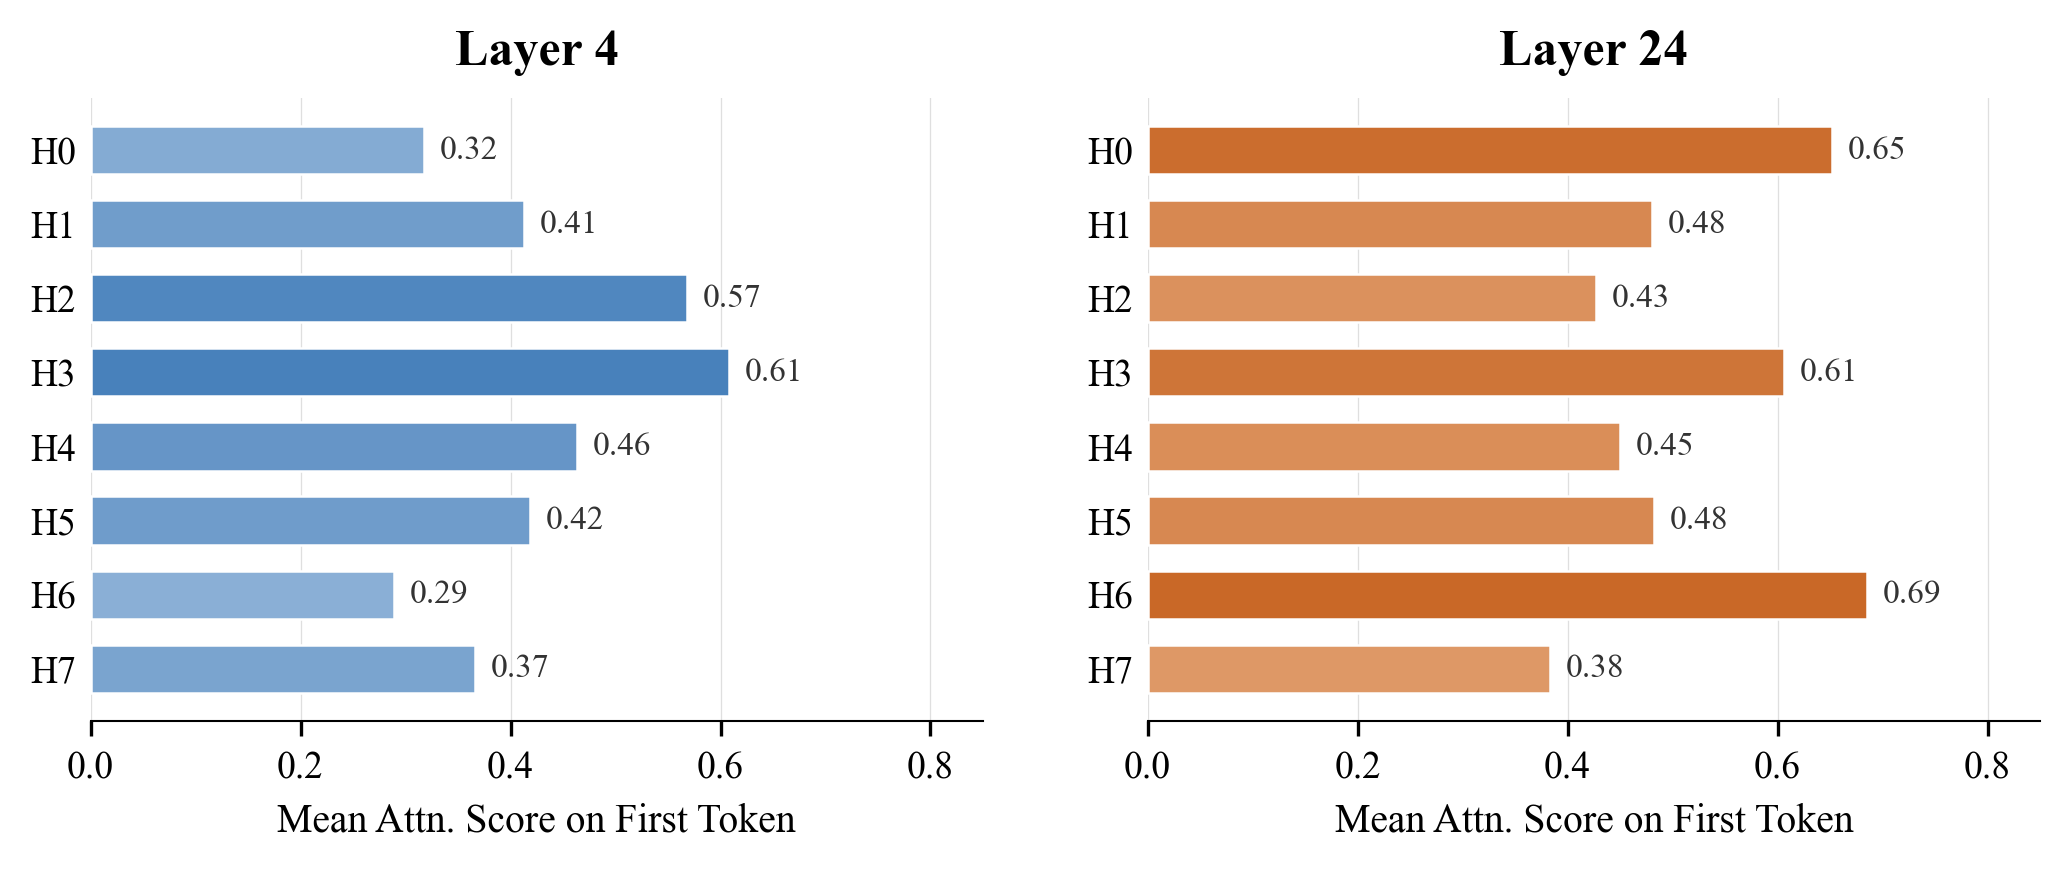
\includegraphics[width=0.92\linewidth]{figures/plot_sink_v2.png}
\caption{Mean attention score on the first token for each attention head in Layer~4 and Layer~24. All heads allocate a significant fraction of attention to the first token, confirming a pervasive attention sink effect across heads and layers.}
\label{fig:attention-sink}
\end{figure}

\section{Preliminary Experiments}
\label{app:prelim}

This section presents small-scale ablation studies on a pilot model. Our goal is to identify the training-design choices that are essential for stable optimization and strong downstream performance. These results serve as the empirical basis for the final recipe described in \Secref{sec:method}.

\subsection{Setup}
\label{app:prelim-setup}

All ablations in this section use a 10B-parameter pilot Transformer with the same architecture family as the main paper \method{} model but with 16 layers. The model uses a 200K-token vocabulary and hidden size $d_{\rm model}=2048$. Each attention module uses GQA with 32 query heads, 4 KV heads, head dimension 128, and RoPE dimension 64. The MoE contains 64 experts with top-4 expert routing and expert inner dimension 1536. The model has 10.53B total parameters and 1.47B active parameters per token. The optimizer, learning-rate schedule, and tokenizer match the full-scale configuration. Each run is trained on a subset of the same pretraining corpus used at full scale.


\subsection{Gradient Sources for the Index Branch}
\label{app:prelim-grad-source}

A central challenge in training the Index Branch is that the top-$k$ selection in \Eqref{eq:msa-topk} is non-differentiable. Under the plain sparse-attention forward pass, the selected block indices are used only as a discrete routing decision. Consequently, the index projections $\mW^{\rm idx}_q$ and $\mW^{\rm idx}_k$ receive no useful gradient from the language-modelling objective, and the indexer cannot learn which blocks should be selected.
There are several possible ways to introduce a training signal for the indexer. We investigate two mechanisms that preserve the sparse-attention structure while providing gradients to the Index Branch.

\textbf{Index Branch output.} The first mechanism lets the Index Branch contribute an additional attention output. Specifically, we attach a value projection to the Index Branch and compute $\mO^{\rm idx}=\mathrm{Attn}(\mQ^{\rm idx}, \mK^{\rm idx}, \mV^{\rm idx})\in \mathbb{R}^{N \times H_q \times d_h}$. This output is added to the layer output through a separate output projection, $\mO'=\mW_o \mO+\mW^{\rm idx}_o \mO^{\rm idx}$. 
This design trains the Index Branch through its contribution to next-token prediction.


\textbf{KL loss.} The second mechanism directly supervises the Index Branch by matching its selection distribution to the Main Branch on the selected support. We use the auxiliary loss $\Ls_{\rm KL}$ defined in \Eqref{eq:msa-kl}. This loss acts on $\mW^{\rm idx}_q$ and $\mW^{\rm idx}_k$, and provides an explicit training signal for the index selection. 

To separate the effects of these two gradient sources, we train the model from scratch in three configurations, using sparse attention from the first step:
\begin{itemize}
    \item \textbf{LM Loss only}: the Index Branch output is added to the layer output, and the model is trained only with the language-modelling loss,
    \begin{equation}
    \mO' = \mW_o \mO + \mW^{\rm idx}_o \mO_{\rm idx},
    \qquad
    \Ls = \Ls_{\rm LM}.
    \end{equation}

    \item \textbf{KL Loss only}: the Index Branch output is discarded, and the indexer is trained only through the auxiliary KL loss,
    \begin{equation}
    \mO' = \mW_o \mO,
    \qquad
    \Ls =\Ls_{\rm LM}+\lambda \sum_{\rm layers} \Ls_{\rm KL}.
    \end{equation}

    \item \textbf{LM Loss\,+\,KL Loss}: both mechanisms are enabled,
    \begin{equation}
    \mO' = \mW_o \mO + \mW^{\rm idx}_o \mO_{\rm idx},
    \qquad
    \Ls =\Ls_{\rm LM}+\lambda \sum_{\rm layers} \Ls_{\rm KL}.
    \end{equation}
\end{itemize}

\Figref{fig:prelim-grad-source} reports the per-benchmark delta of each configuration against the Full-Attention GQA baseline trained on the same data. The two single-signal configurations show complementary weaknesses. \textbf{LM Loss only} preserves short-context ability but performs poorly on long-context retrieval: without an objective on the top-$k$ selection itself, the indexer receives little direct pressure to select relevant blocks. \textbf{KL Loss only} improves retrieval but reduces short-context ability: removing $\mO_{\rm idx}$ from the layer output reduces the attention capacity available to the language model. \textbf{LM Loss\,+\,KL Loss} gives the best balance across the two axes and is the configuration we use for the remaining ablations in this section.

\begin{figure}[!htb]
\centering
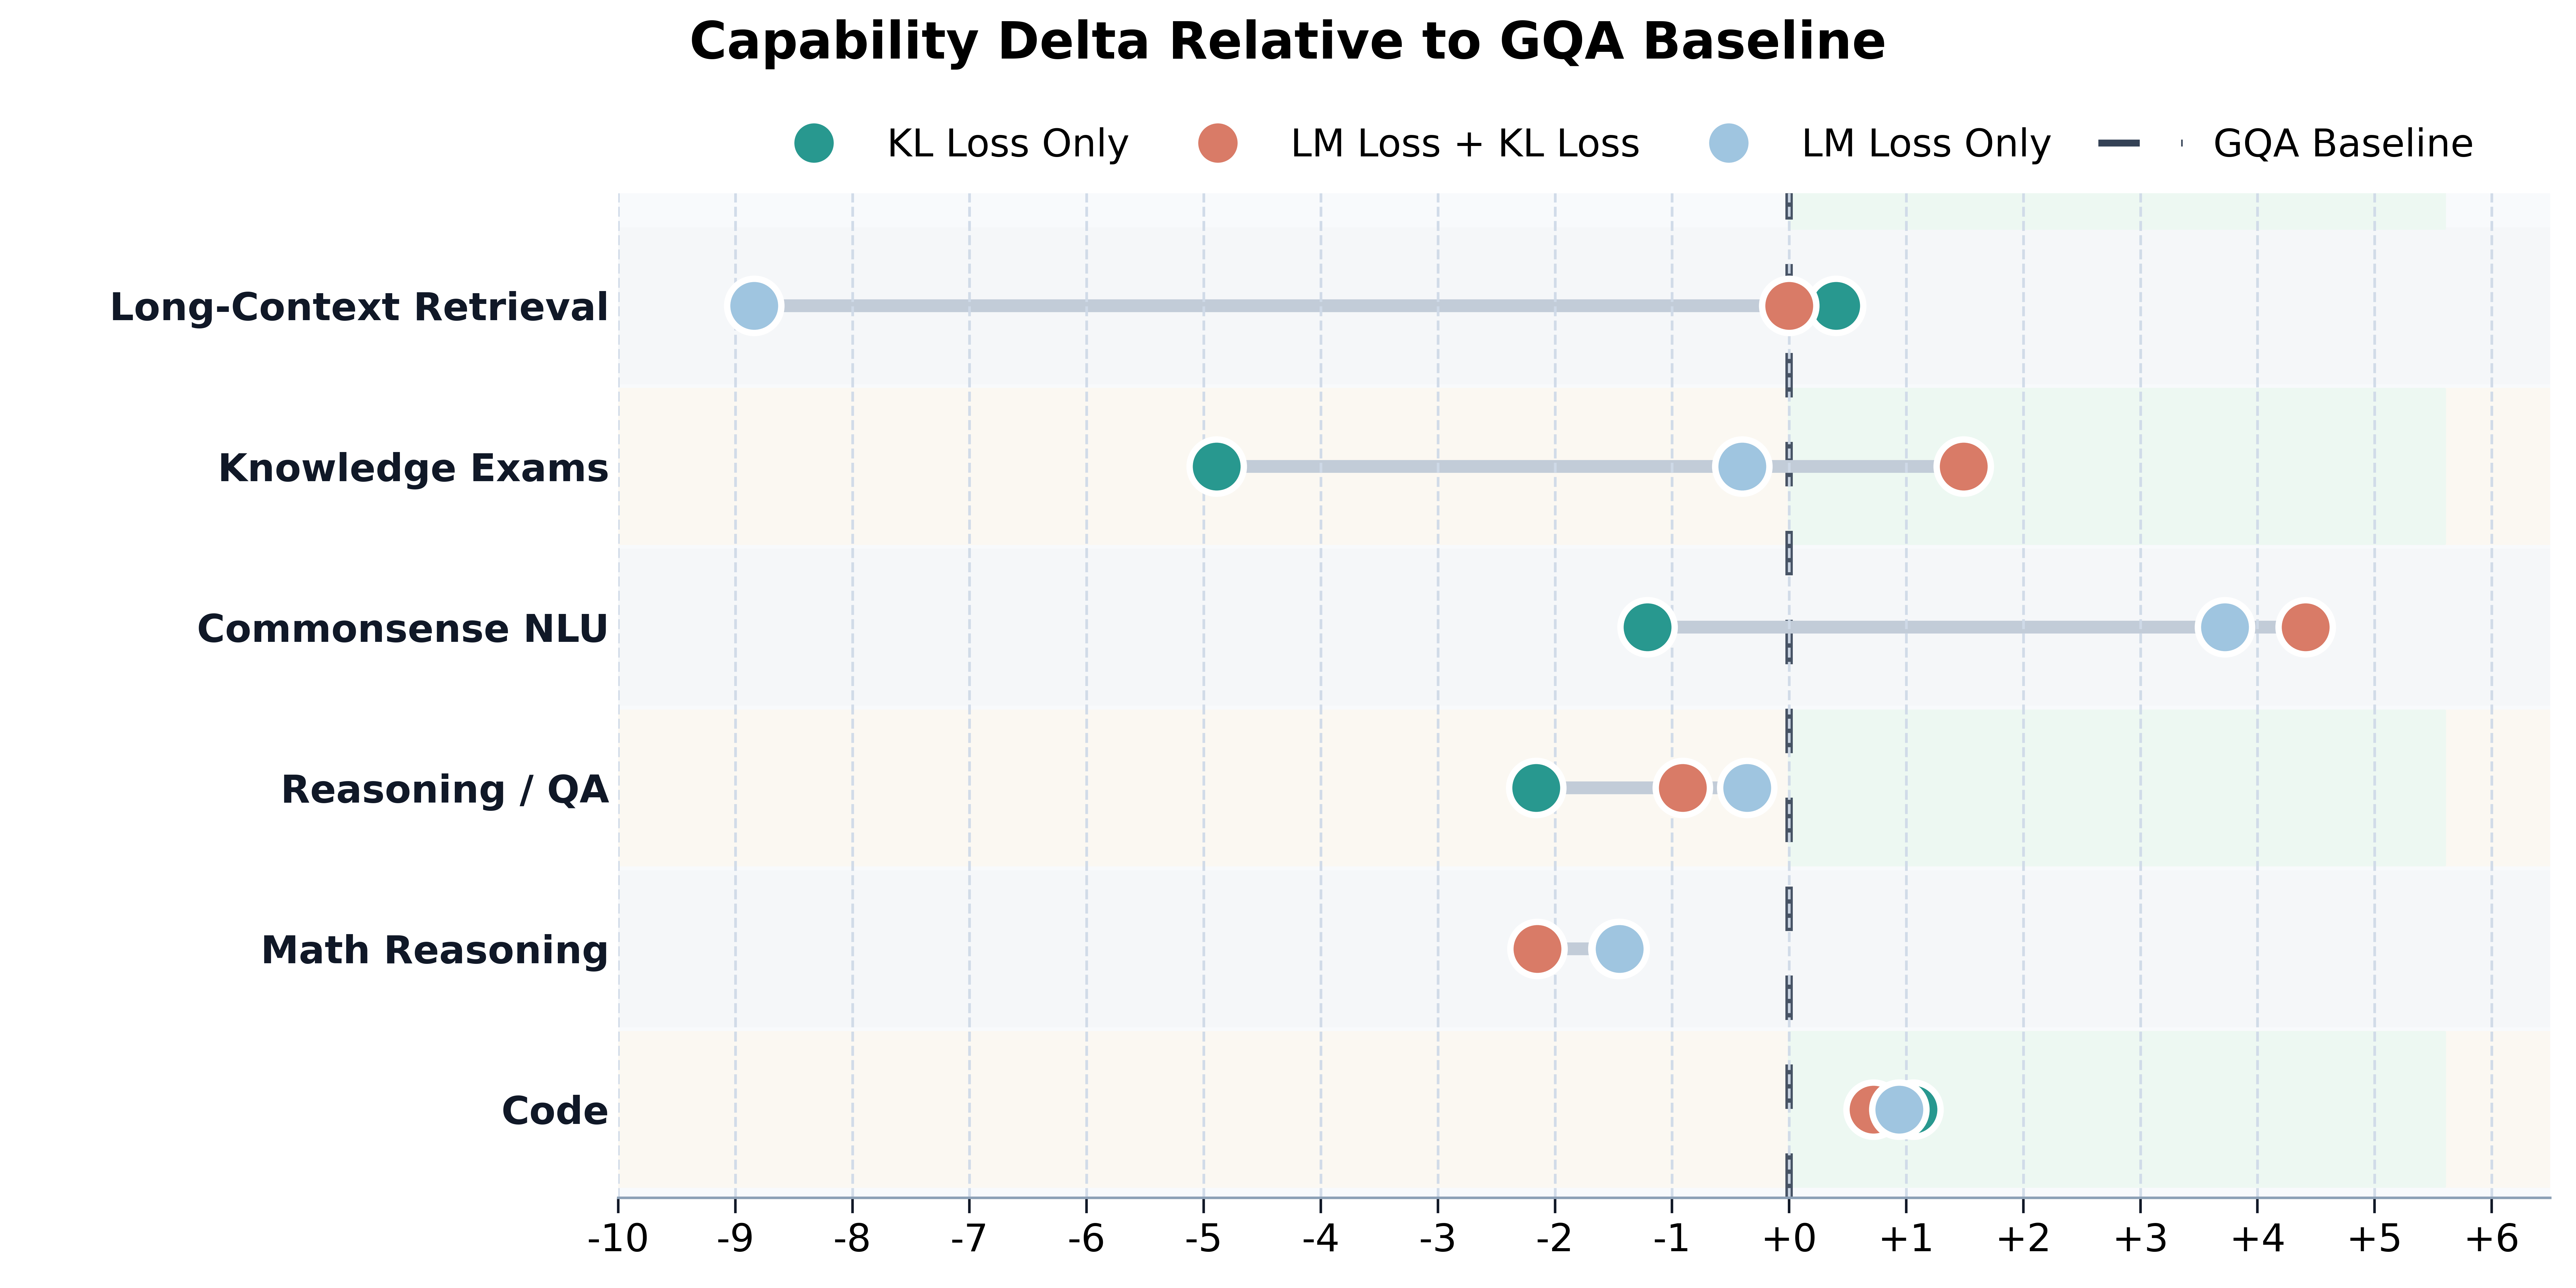
\includegraphics[width=0.85\linewidth]{figures/idx_grad_1.png}
\caption{Evaluation-score deltas relative to the Full-Attention
baseline for three indexer training signals in the pilot setting.
Positive values indicate improvements over the baseline, and negative
values indicate degradations.}
\label{fig:prelim-grad-source}
\end{figure}

Based on these results, we use the \textbf{LM Loss\,+\,KL Loss} configuration for the remaining ablations in this section. We later show in \Secref{app:from-scratch-no-idx-value} that, once the indexer warmup introduced in \Secref{app:prelim-warmup} is used in the full-scale setting, the Index Branch output is no longer necessary. The final recipe, therefore, keeps the KL supervision but removes the Index Branch value head and its additive output path.

\subsection{Confining the KL Gradient to the Index Branch}
\label{app:prelim-detach}


The auxiliary KL loss is intended to train the Index Branch to match the Main Branch selection distribution. Under the default autograd graph, the KL gradient flows through the Index Branch query and key projections back into the hidden state, and then into the backbone through the residual stream. In this case, the KL loss becomes an additional objective on the backbone, rather than a local supervision signal for the indexer.

We observe two failure modes from this gradient routing. With larger KL coefficients, occasional KL-gradient spikes propagate into the backbone, causing gradient-norm spikes and LM-loss divergence within a few hundred steps (\Figref{fig:prelim-detach}). Even at stable coefficients, standard short-context benchmarks gradually regress during training (\Figref{fig:prelim-detach-bench}). We attribute this regression to a self-distillation effect: the backbone can lower the KL loss by simplifying the Main Branch attention distribution, rather than by improving the Index Branch.

We address both failure modes by stopping the KL gradient at the Index Branch input (\Secref{sec:method-training}). Thus, each layer's KL loss becomes a local supervision signal for its own indexer. With this detach, the LM loss and gradient norm remain stable under the same KL coefficients that cause divergence without detach (\Figref{fig:prelim-detach}), and the short-context regression is removed (\Figref{fig:prelim-detach-bench}). We use this detach in all subsequent runs.

\begin{figure}[!htb]
\centering
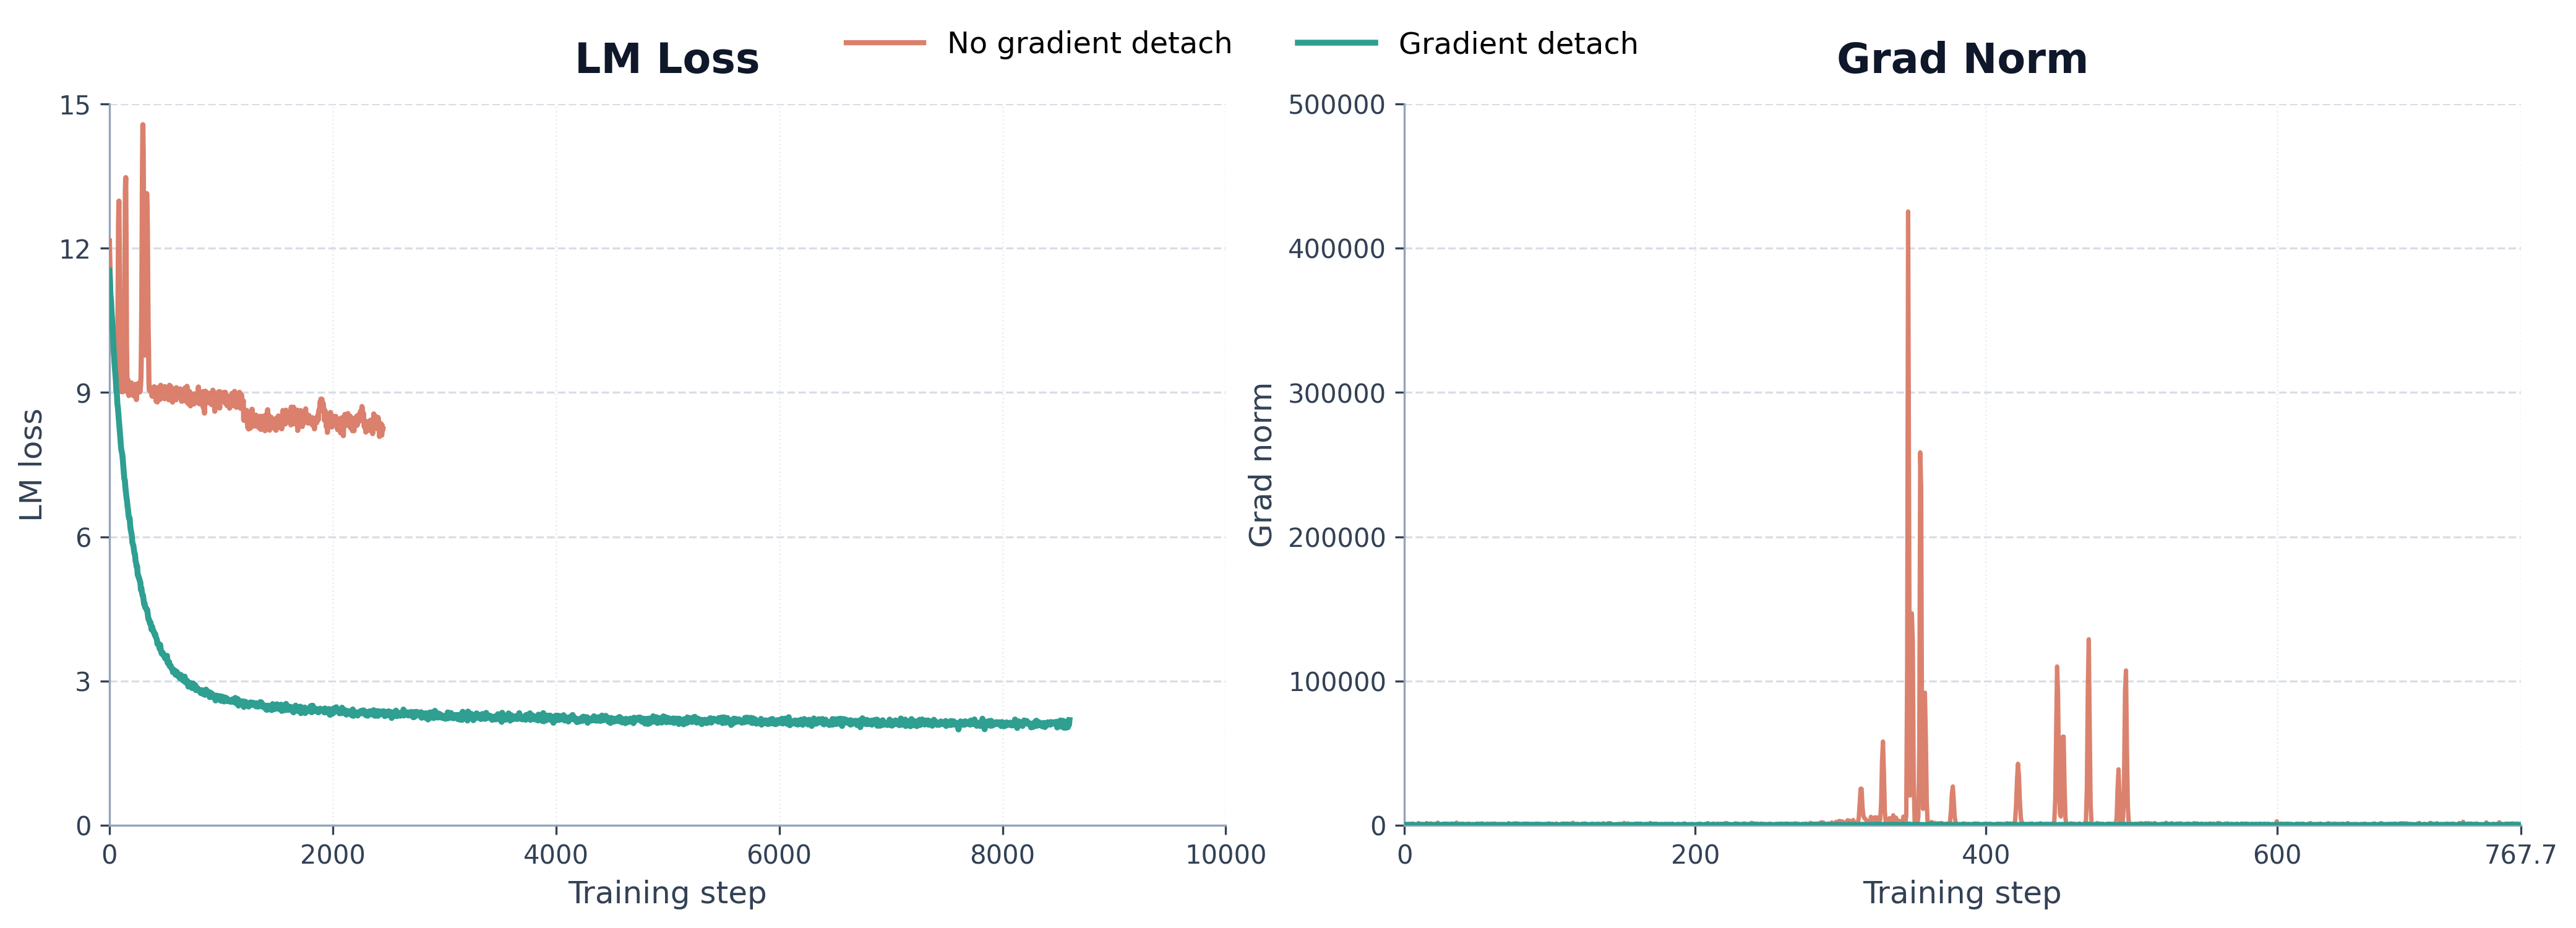
\includegraphics[width=0.85\linewidth]{figures/loss_gradnorm_replica.png}
\caption{
Training LM loss and gradient norm with and without detaching the KL gradient from the backbone. Detaching confines the auxiliary loss to the Index Branch and avoids the gradient spikes observed without detach.
}
\label{fig:prelim-detach}
\end{figure}

\begin{figure}[!htb]
\centering
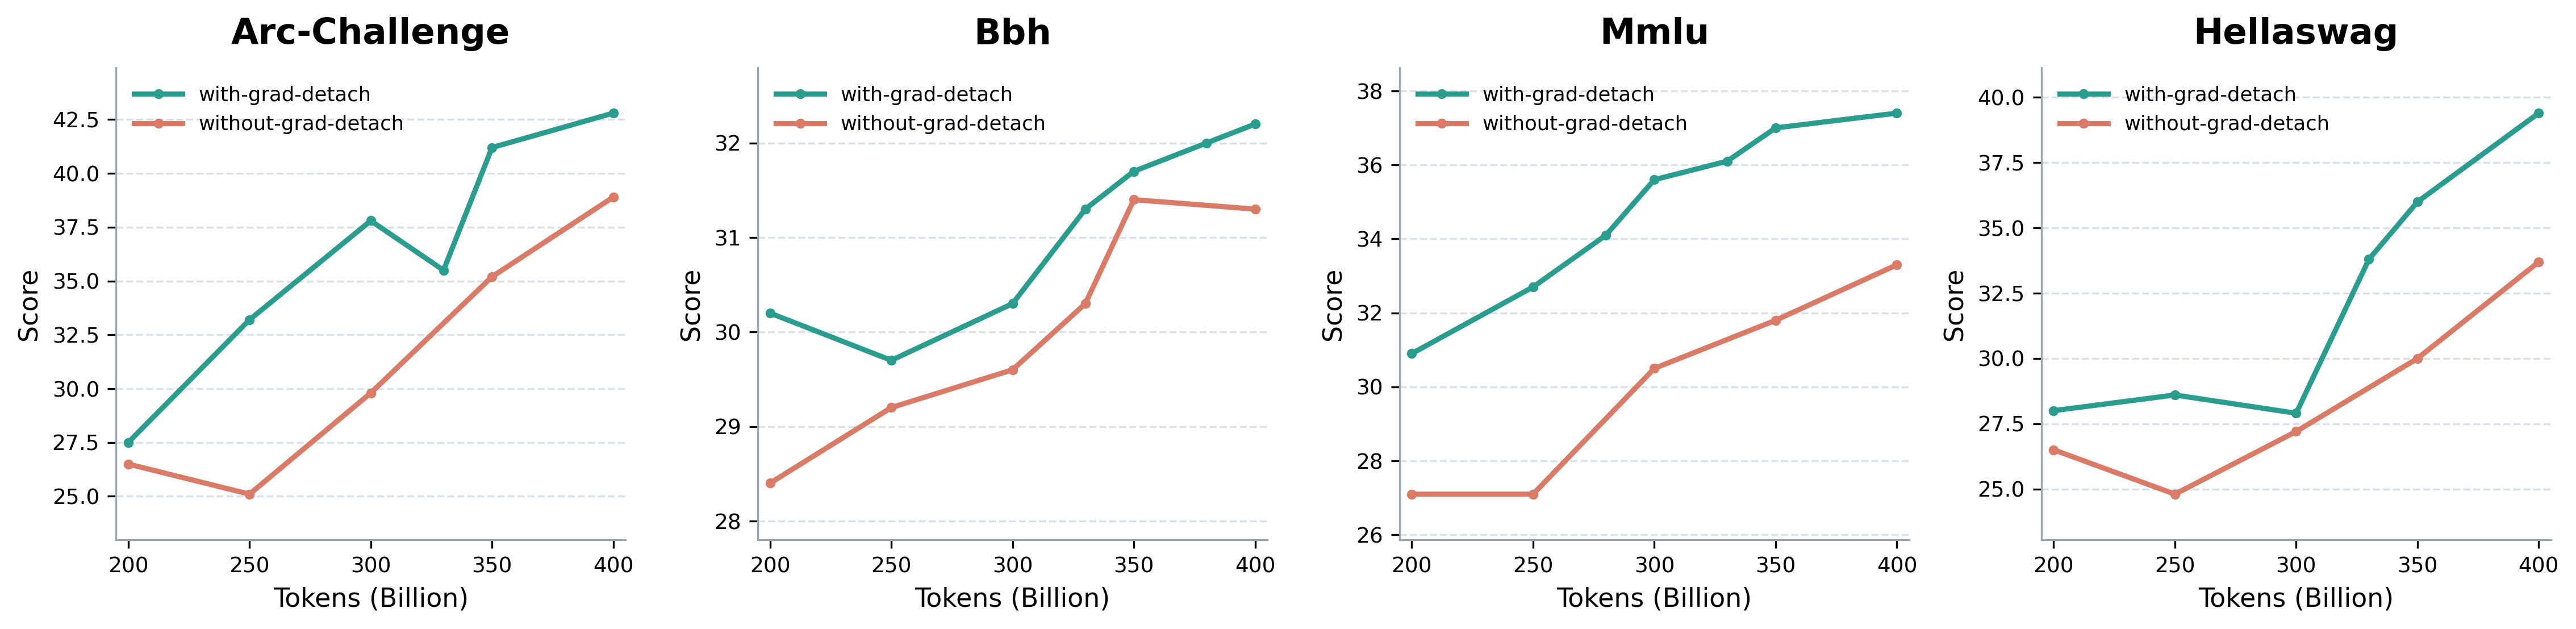
\includegraphics[width=0.8\linewidth]{figures/redrawn_four_benchmarks.png}
\caption{
General benchmark scores with and without detaching the KL gradient from the backbone. Detaching the auxiliary loss reduces the general ability degeneration observed when the KL gradient updates the backbone.
}
\label{fig:prelim-detach-bench}
\end{figure}


\subsection{Indexer Warmup}
\label{app:prelim-warmup}

We observe that the Main Branch attention distribution changes rapidly during the earliest stage of training. As shown in \Figref{fig:prelim-warmup-entropy}, the attention entropy quickly drops from an initially smooth distribution to a much sharper one, before entering a slower phase of representation learning. This makes sparse selection fragile at initialization. If top-$k$ selection is enabled from step zero, the Index Branch must track a rapidly moving target while its own selections are still nearly random. Poor early selections then route the Main Branch to uninformative tokens, which weakens both backbone learning and the KL supervision received by the indexer.

We address this issue with a short indexer warmup. During warmup, the Main Branch uses full attention, while the Index Branch is trained by the KL loss against the full-sequence Main Branch distribution. This allows the backbone to pass through the early sharpening phase without sparse routing errors, and gives the indexer a meaningful initialization before it controls token selection. After $T_{\rm warm}$ steps, we enable top-$k$ sparse selection and continue training with the KL loss restricted to the selected support.

\Figref{fig:prelim-warmup-curves} compares pretraining runs with and without this warmup. The warmed-up run achieves better short-context performance and stronger long-context retrieval. These results indicate that a short full-attention warmup provides a better initialization for sparse training. We therefore also adopt this warmup when converting Full-Attention checkpoints to sparse attention through continued pretraining.

\begin{figure}[!htb]
\centering
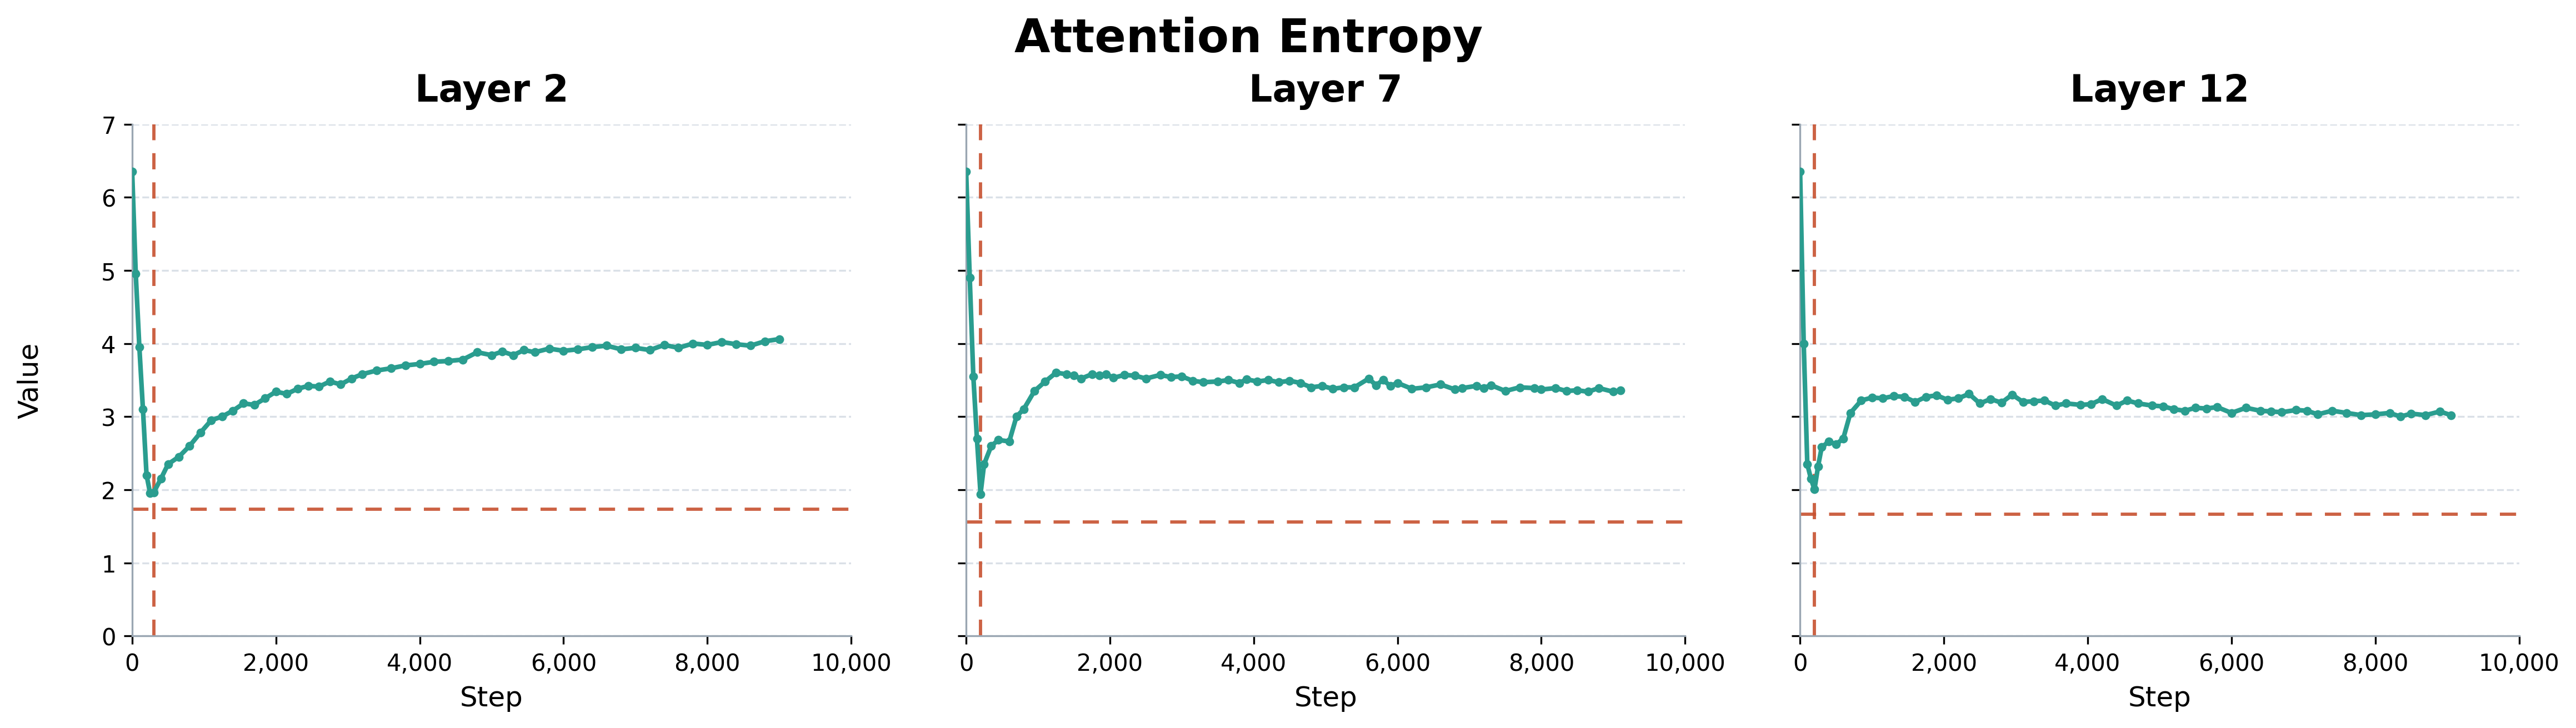
\includegraphics[width=0.85\linewidth]{figures/redrawn_layers_2_7_12.png}
\caption{Per-layer entropy of the Main Branch attention distribution
during early sparse training. Entropy drops rapidly in the first few
hundred steps before partially recovering and stabilizing, motivating a
brief full-attention warmup for the indexer.}
\label{fig:prelim-warmup-entropy}
\end{figure}

\begin{figure}[!htb]
\centering
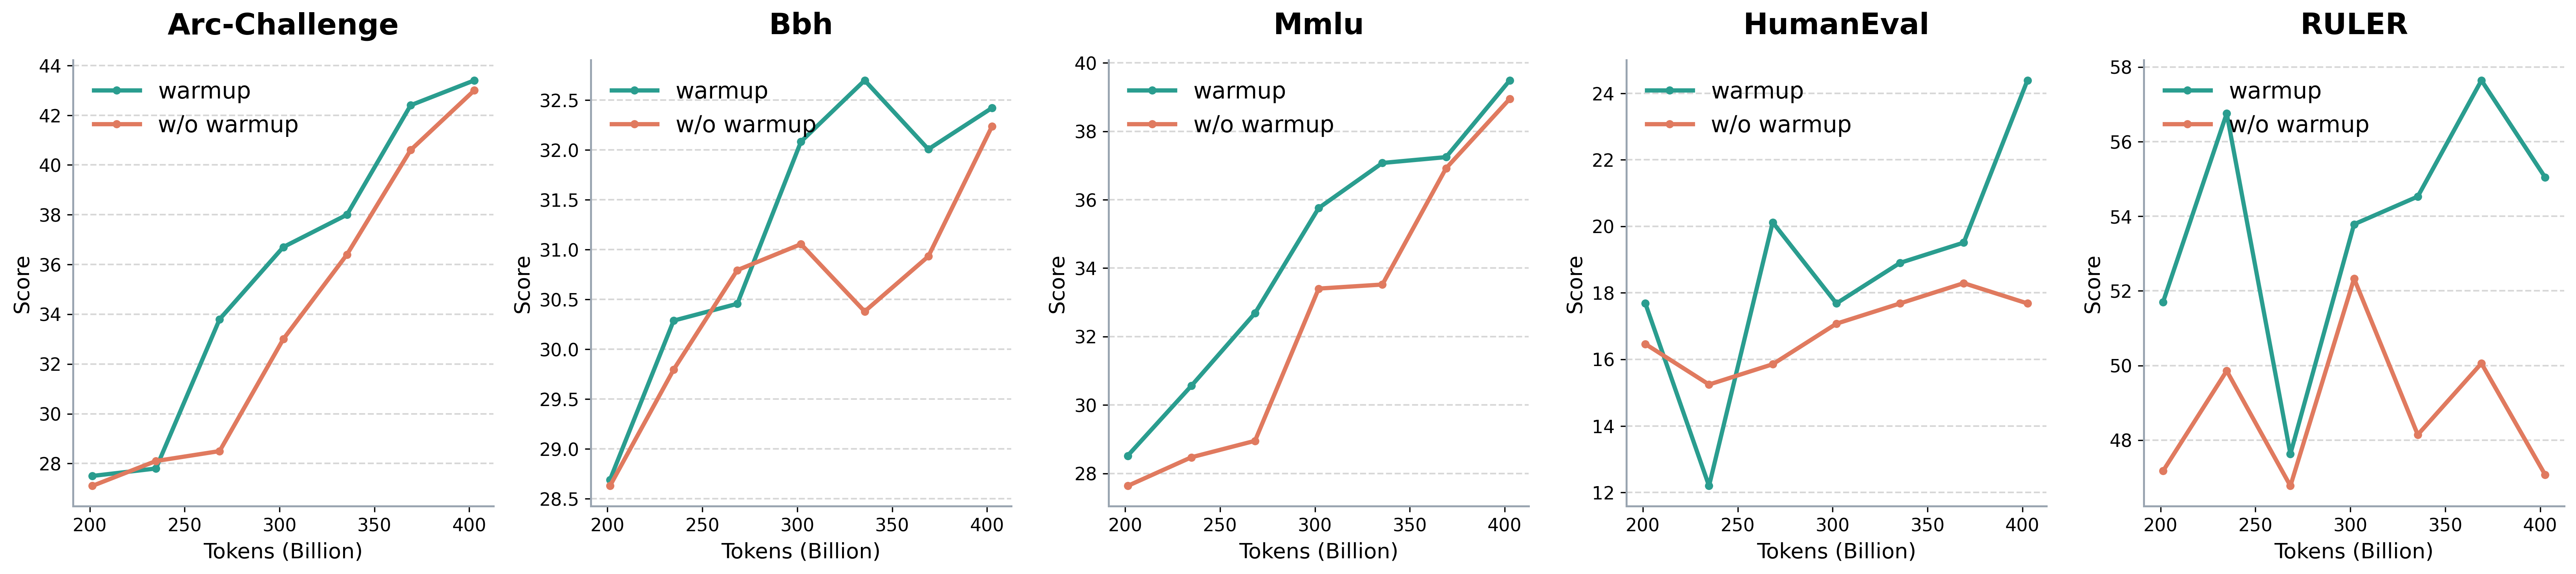
\includegraphics[width=0.98\linewidth]{figures/msa_curves_reproduce.png}
\caption{Evaluation results of \method{} with and without index warmup. Within the reported training range, index warmup improved scores on general tasks and long-context retrieval.}
\label{fig:prelim-warmup-curves}
\end{figure}



\subsection{Learnable Attention Sink}
\label{app:prelim-learnable-sink}

The visualization in \Figref{fig:attention-sink} shows that the first token often acts as an attention sink: many heads assign a non-trivial amount of attention mass to the sequence prefix, even when the sparse selector is not explicitly forced to include it. This raises the question of whether this sink behavior should be represented by an explicit learnable mechanism, rather than being absorbed by the first real token in the sequence.
We therefore tested a GPT-OSS-style learnable attention sink. Concretely, each attention head is given an additional learnable sink logit, which competes with normal key positions in the attention softmax.

\Figref{fig:prelim-learnable-sink-vis} visualizes the resulting attention patterns. The learnable sink absorbs substantial attention mass in some heads, but it does not completely remove the original first-token sink. In several heads, especially those where the learned sink receives little mass, the first token still receives substantial attention and continues to behave as an implicit sink.

\begin{figure}[!htb]
\centering
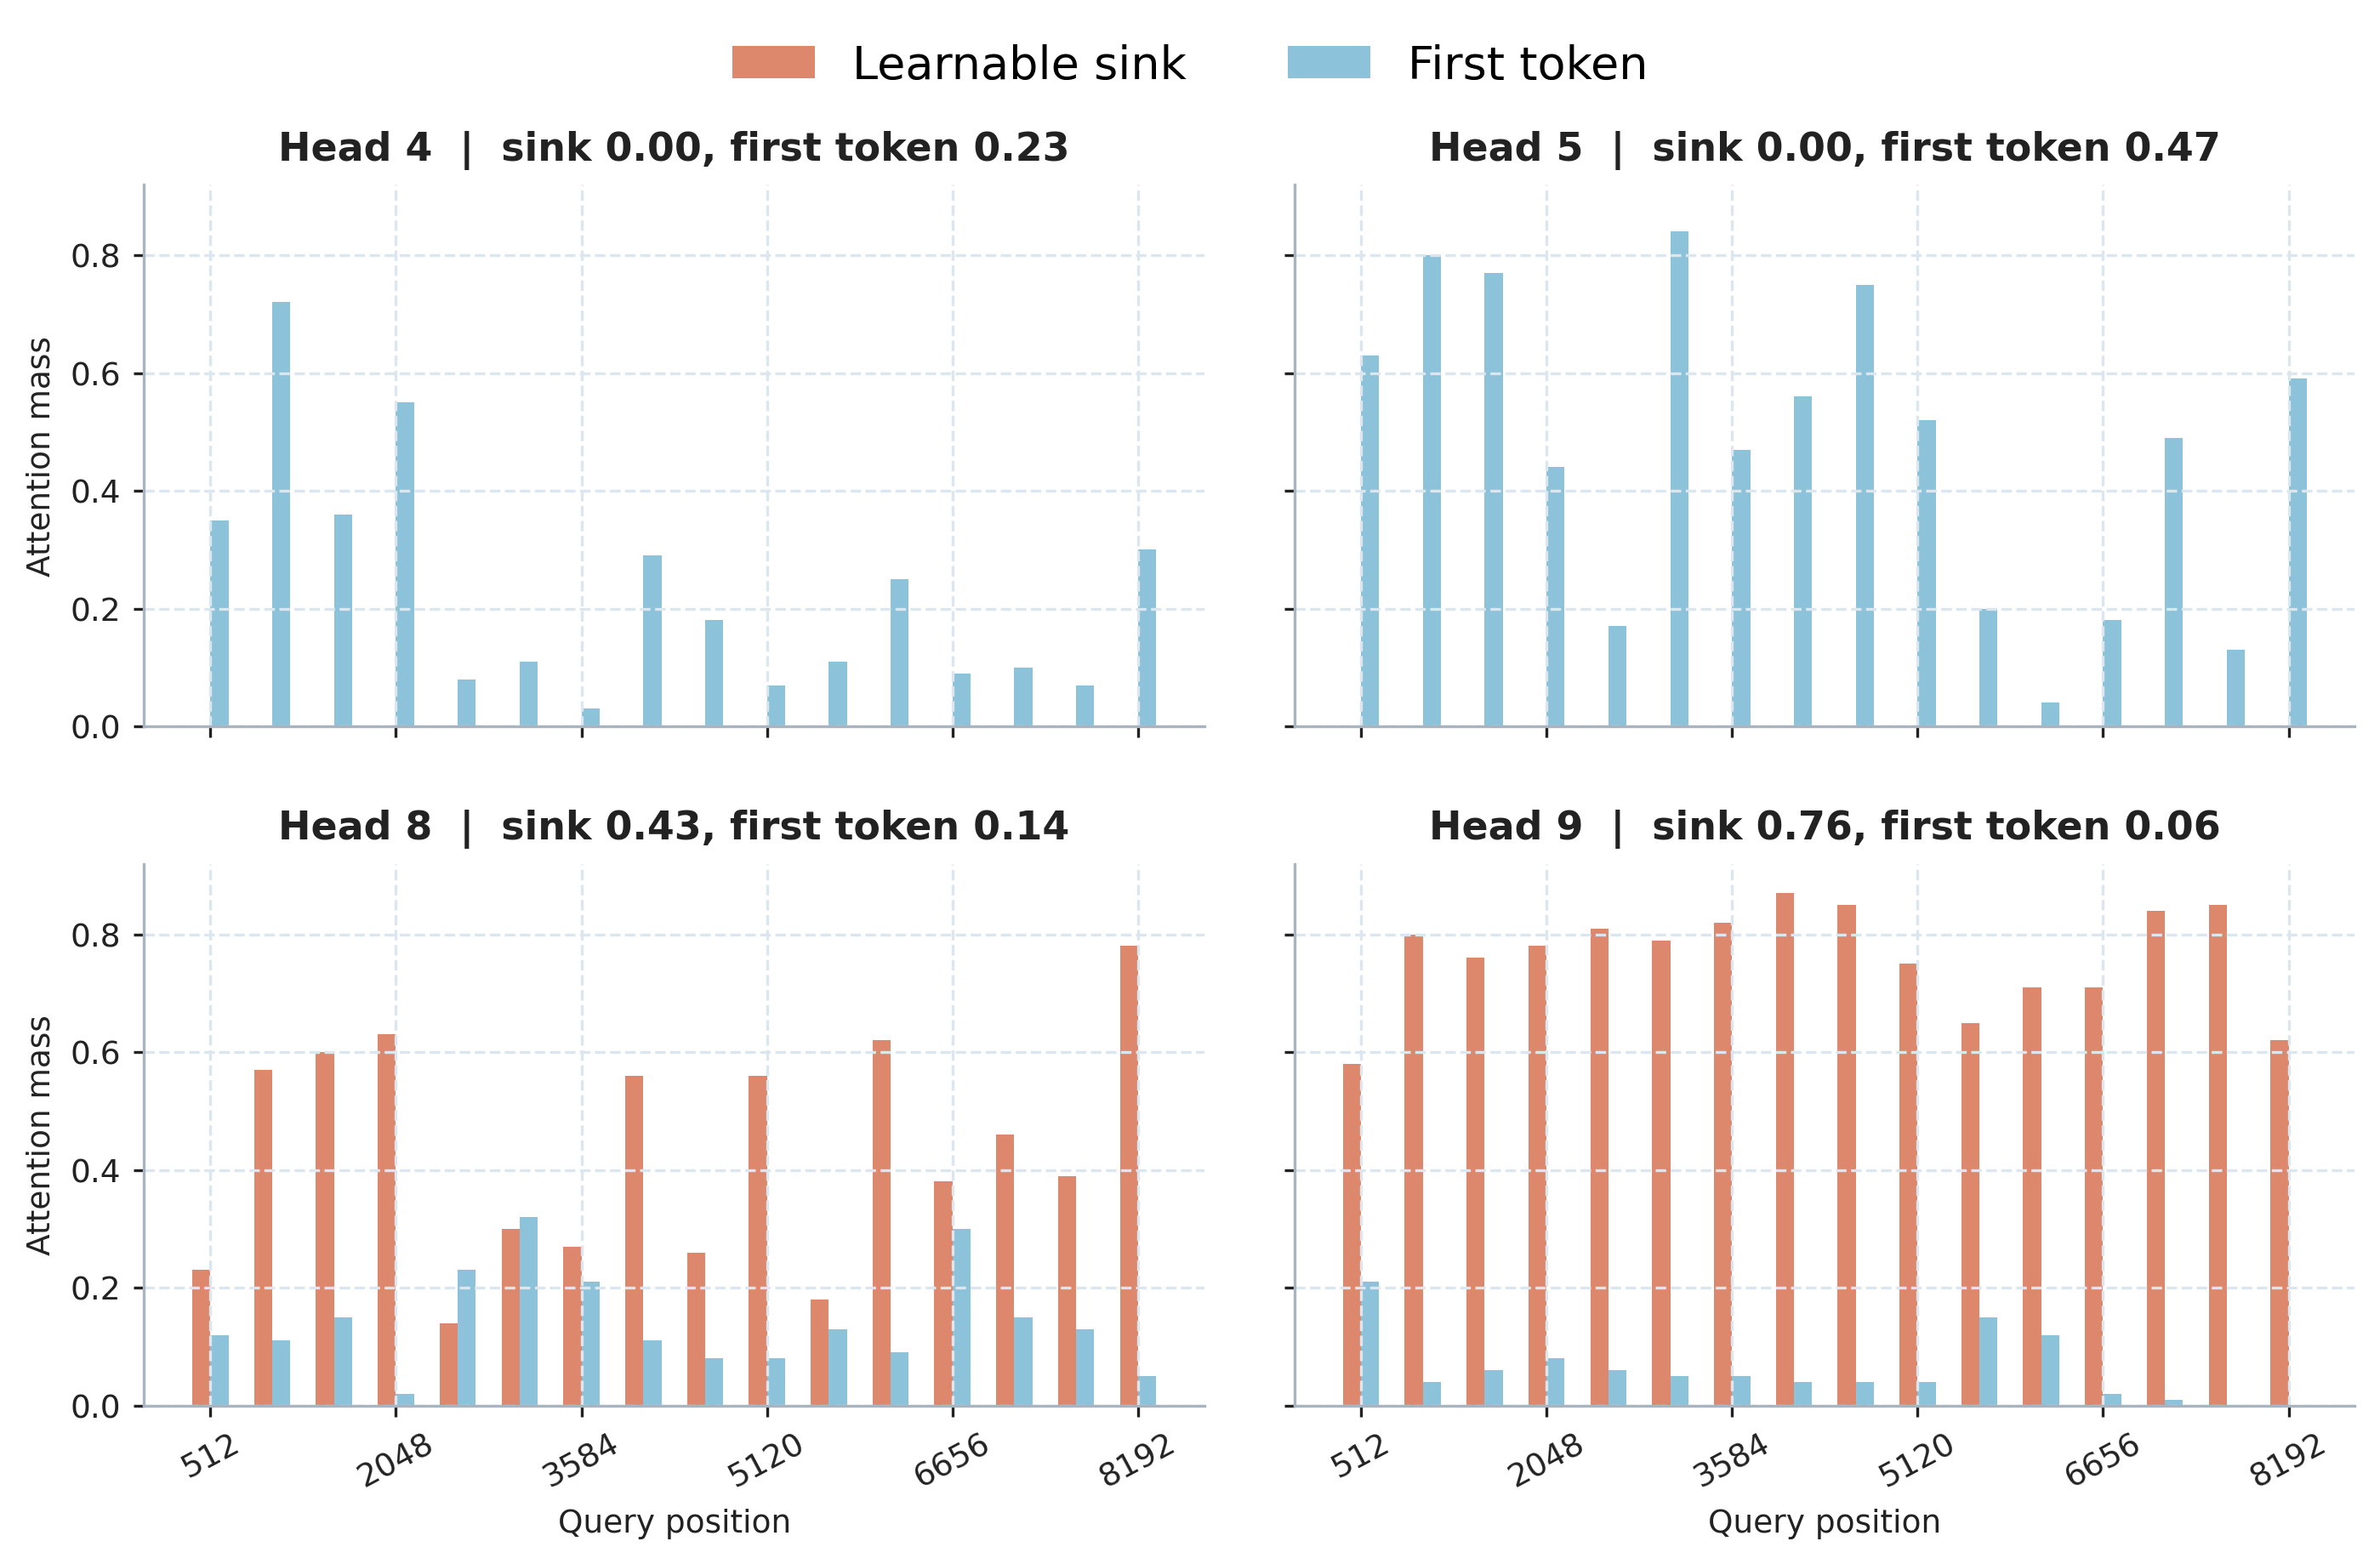
\includegraphics[width=0.92\linewidth]{figures/learnable_sink_vis.png}
\caption{Attention received by the learnable sink and the first token after introducing a GPT-OSS-style sink parameter. In some heads, the learnable sink absorbs most of the sink-like attention; in others, the first token remains the dominant sink, indicating that the explicit sink does not fully eliminate first-token sink behavior.}
\label{fig:prelim-learnable-sink-vis}
\end{figure}

We also compare downstream perplexity with and without the learnable sink in \Figref{fig:prelim-learnable-sink-results}. The learnable-sink variant does not yield a clear or consistent improvement over the default design. Given its additional parameters, implementation complexity, and the fact that it does not fully suppress first-token sink behavior, we do not include the learnable attention sink in the final recipe.

\begin{figure}[!htb]
\centering
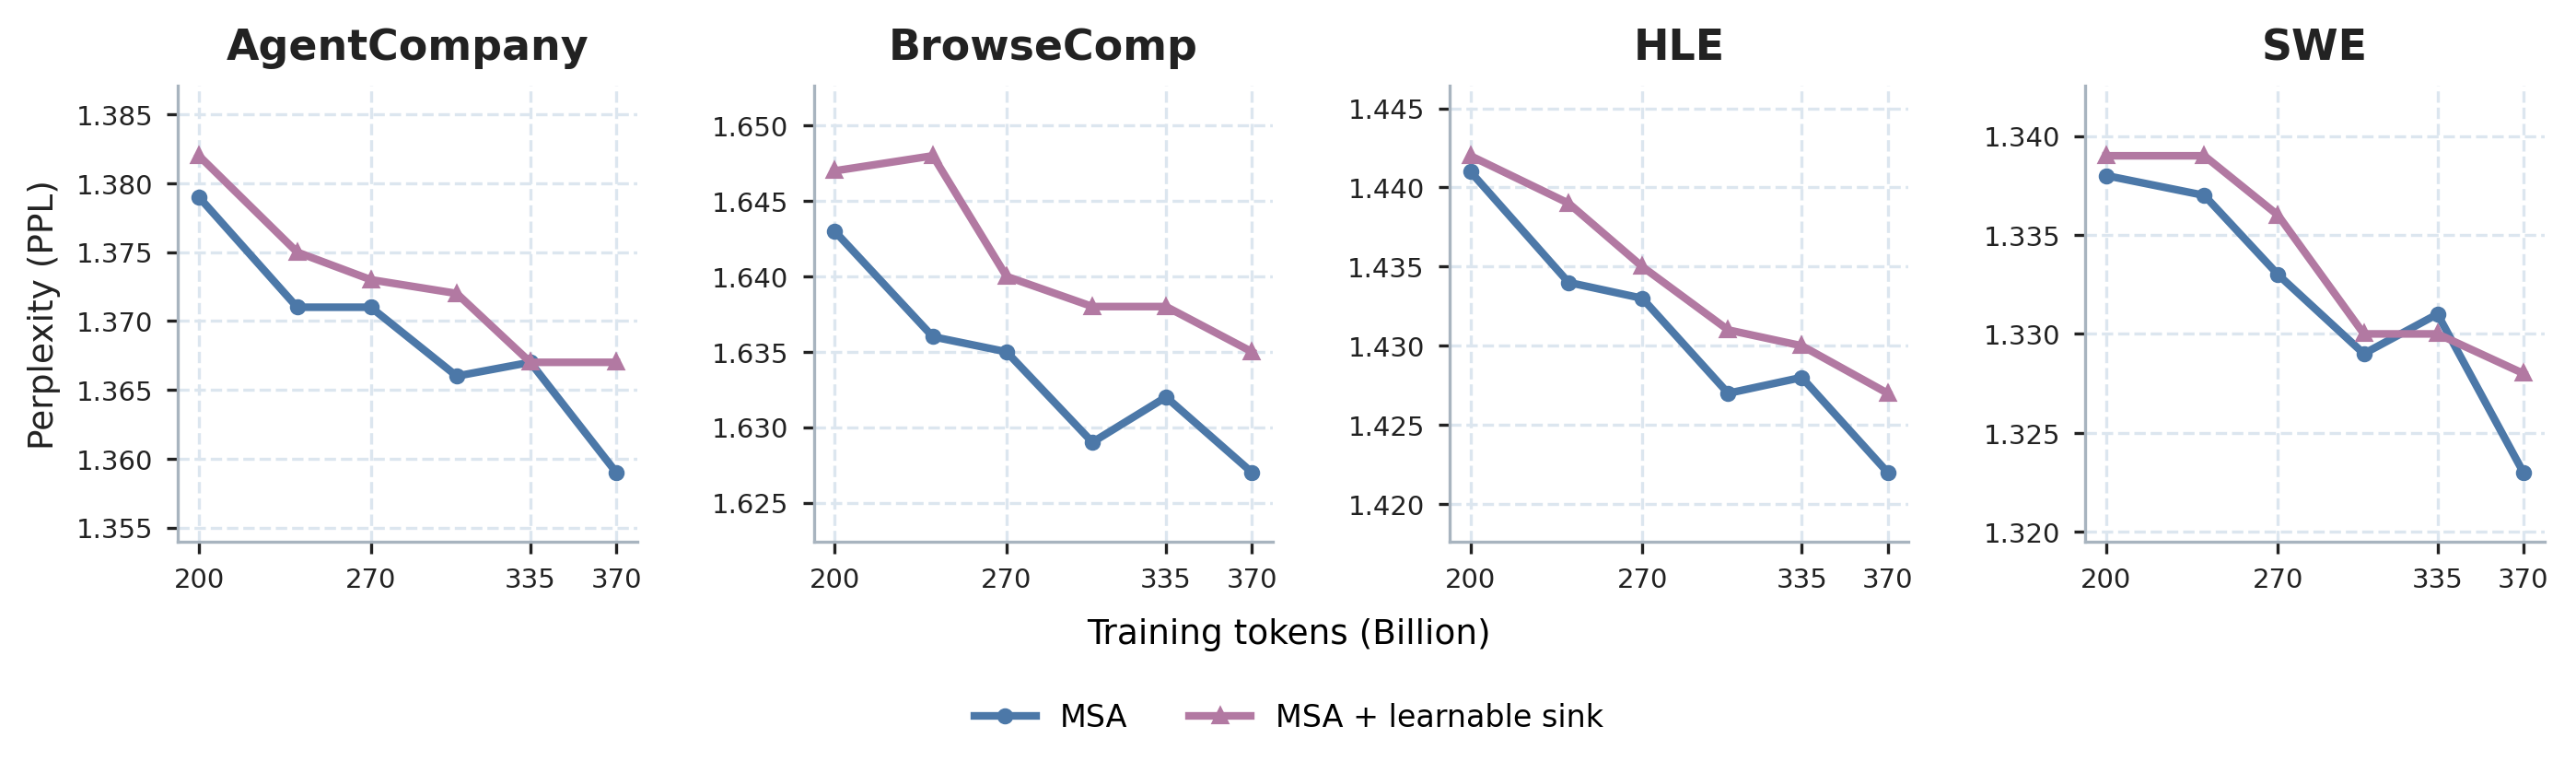
\includegraphics[width=0.85\linewidth]{figures/learnable_sink_results.png}
\caption{Perplexity comparison with and without the learnable attention sink on downstream agent-oriented evaluations. Lower perplexity is better. Adding the learnable sink does not provide a consistent advantage over the default \method{} design.}
\label{fig:prelim-learnable-sink-results}
\end{figure}


\subsection{Dynamic Sparse Selection vs.\ Sliding Window}
\label{app:prelim-swa}

To assess the value of dynamic selection, we compare \method{} with a FLOP-matched sliding-window baseline. This baseline removes the Index Branch and uses a fixed sparse pattern: each query attends to the first key block and to a local window with the same token budget ending at the query. Therefore, the two methods have the same selection budget and differ only in whether the selected tokens are fixed by position or chosen dynamically.

Figure~\ref{fig:prelim-swa-ppl} reports perplexity on downstream agent tasks. Under the same sparse selection budget, the sliding-window model has higher perplexity than \method{} across the training trajectory. Although both models benefit from additional training tokens, the fixed local-window pattern does not match the perplexity of dynamic sparse selection. This suggests that, for these agent tasks, a position-fixed sparse pattern is less suitable than content-dependent token selection.


\begin{figure}[!htb]
\centering
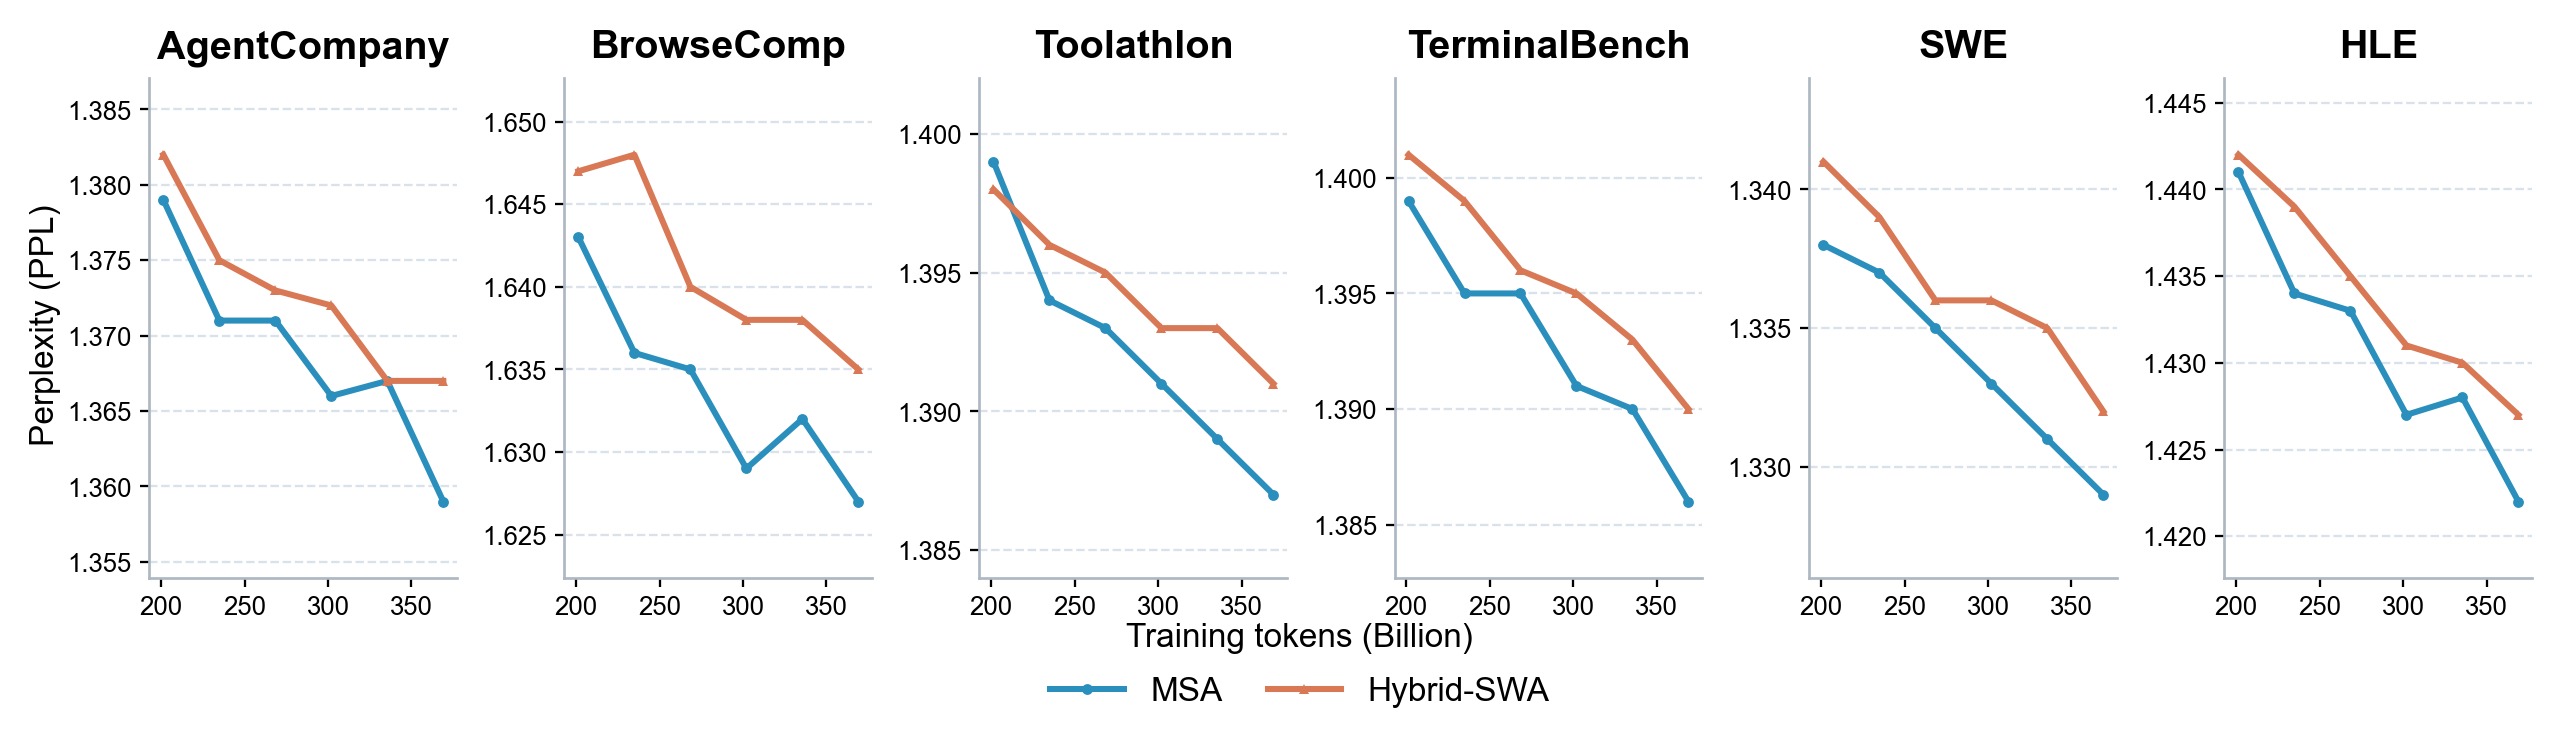
\includegraphics[width=0.9\linewidth]{figures/abaltion_swa_ppl.png}
\caption{Perplexity comparison between \method{} and a FLOP-matched
sliding-window baseline on downstream agent-oriented evaluations. Lower
Perplexity indicates better modeling performance under the same sparse
selection budget.}
\label{fig:prelim-swa-ppl}
\end{figure}


\section{Additional Ablation Study}
\label{app:additional-ablation}


\subsection{Block Size}
\label{app:prelim-block-size}

The sparse attention calculation in \method{}'s Main Branch processes key-value pairs in units of consecutive $B_k$ token blocks, which affects both model performance and efficiency. Larger blocks can improve kernel efficiency but may reduce retrieval quality because of coarser selection granularity. By adjusting $B_k$ while keeping the total number of selected tokens constant, we investigate this trade-off. Compared to the main experiment, these runs use fewer training iterations and a subset of the evaluation suite.

As shown in Table~\ref{tab:block-ablation}, varying the block size has a limited impact on model quality in this setting. The PPL results are nearly unchanged across different $B_k$ values, and the RULER scores show no clear degradation when increasing the block size from 32 to 64 or 128. This suggests that \method{} can use larger key-value blocks to improve kernel efficiency with limited quality loss in these ablations.

\begin{table}[!htb]
\centering
\caption{Perplexity and long-context retrieval scores for different
key-value block sizes. Lower is better for perplexity, and higher is
better for RULER scores.}
\label{tab:block-ablation}
\small
\begin{tabular}{l c c c}
\toprule
Benchmark & Block 32 & Block 64 & Block 128 \\
\midrule
\multicolumn{4}{l}{\textit{PPL $\downarrow$}} \\
TAU2                             & 1.176 & 1.176 & 1.176 \\
AgentCompany                     & 1.266 & 1.276 & 1.266 \\
HLE                              & 1.299 & 1.299 & 1.300 \\
SWE                              & 1.233 & 1.233 & 1.233 \\
\midrule
\multicolumn{4}{l}{\textit{Long-context retrieval}} \\
RULER-8K                          & 72.5 & 72.8 & 73.8 \\
RULER-32K                          & 66.1 & 65.3 & 64.6 \\
\bottomrule
\end{tabular}
\end{table}



\subsection{Forced Sink \& Local Selection}
\label{app:prelim-sink-local}

In early sparse-training experiments, we explicitly forced the selector to include two types of blocks: the first block in the sequence and a fixed local window around the query position. The first block corresponds to the common attention-sink pattern, while the local window preserves nearby context that is important for short-range modeling and provides dense supervision for the indexer. This design was mainly introduced as a stabilization mechanism: before the indexer becomes reliable, forcing these blocks reduces the chance that the sparse branch misses basic context during early training.

We later found that these priors do not need to be hard-coded. When the forced selection of the first block and the fixed local window are removed, the trained model still exhibits both structures: attention concentrates on the sequence prefix when useful, and nearby tokens remain frequently selected.
As shown in Table~\ref{tab:forced-sink-local}, removing forced sink and fixed local selection has little effect on standard model quality: reasoning, code, and PPL metrics remain nearly unchanged. Long-context retrieval is also comparable.
These results indicate that the sparse model can learn sink and local-selection patterns without hard-coded selection rules. Therefore, the final recipe does not force the first block or a large local window, and only forces the special incomplete self block.



\begin{table}[!htb]
\begin{minipage}[t]{0.48\textwidth}
\centering
\caption{Ablation of forced sink and local-window selection. Higher is better unless marked $\downarrow$.}
\label{tab:forced-sink-local}
\small
\begin{tabular}{l c c}
\toprule
Benchmark & No Forced & Forced \\
\midrule
\multicolumn{3}{l}{\textit{General knowledge \& reasoning}} \\
MMLU                                & 60.5 & 60.5 \\
MMLU-Pro                            & 32.5 & 33.4 \\
BBH                                 & 58.2 & 58.2 \\
ARC Challenge                       & 78.1 & 77.9 \\
\midrule
\multicolumn{3}{l}{\textit{Math}} \\
GSM8K                               & 66.0 & 66.9 \\
MGSM                                & 35.8 & 36.3 \\
\midrule
\multicolumn{3}{l}{\textit{Code}} \\
EvalPlus                            & 54.0 & 53.6 \\
BigCodeBench                        & 35.6 & 35.7 \\
MultiPL-E MBPP P@10                 & 80.1 & 79.5 \\
\midrule
\multicolumn{3}{l}{\textit{Image}} \\
ChartQA                            & 73.5 & 73.7 \\
MMMU                               & 43.6 & 42.9 \\
\midrule
\multicolumn{3}{l}{\textit{Video}} \\
VideoMMMU                          & 32.1 & 32.0 \\
\midrule
\multicolumn{3}{l}{\textit{PPL $\downarrow$}} \\
TAU2                                & 1.175 & 1.175 \\
AgentCompany                        & 1.268 & 1.266 \\
HLE                                 & 1.301 & 1.300 \\
SWE                                 & 1.235 & 1.233 \\
\midrule
\multicolumn{3}{l}{\textit{Long-context retrieval}} \\
RULER-8K                             & 71.6 & 71.7 \\
RULER-32K                            & 61.5 & 65.8 \\
\bottomrule
\end{tabular}
\end{minipage}\hfill
\begin{minipage}[t]{0.46\textwidth}
\centering
\caption{Continued pre-training ablation of the Index Branch value head.}
\label{tab:idxval-ablation}
\small
\begin{tabular}{l c c}
\toprule
Benchmark & With-value & No-value \\
\midrule
\multicolumn{3}{l}{\textit{General knowledge \& reasoning}} \\
MMLU                                & 66.4 & 67.3 \\
MMLU-Pro                            & 39.0 & 39.1 \\
BBH                                 & 65.3 & 65.9 \\
ARC Challenge                       & 82.2 & 82.4 \\
\midrule
\multicolumn{3}{l}{\textit{Math}} \\
GSM8K                               & 77.6 & 76.4 \\
MathVista                           & 45.2  & 43.6  \\
MGSM                                & 48.4 & 47.6 \\
\midrule
\multicolumn{3}{l}{\textit{Code}} \\
HumanEval                           & 60.4 & 59.1 \\
EvalPlus                            & 57.7 & 58.7 \\
BigCodeBench                        & 46.0 & 44.0 \\
\midrule
\multicolumn{3}{l}{\textit{Image}} \\
AI2D                                & 69.3 & 70.4 \\
ChartQA                             & 75.3 & 74.9 \\
MMMU                                & 44.9 & 43.4 \\
OCRBench v2                         & 53.2 & 53.9 \\
\midrule
\multicolumn{3}{l}{\textit{Video}} \\
MLVU                                & 42.4 & 43.9 \\
MMVU                                & 44.9  & 43.7  \\
PerceptionTest                      & 45.0 & 47.3 \\
\midrule
\multicolumn{3}{l}{\textit{Long-context retrieval}} \\
RULER-8K                            & 84.1 & 83.0 \\
RULER-32K                           & 79.7 & 80.4 \\
\bottomrule
\end{tabular}
\end{minipage}
\end{table}


\subsection{Index Branch Value Head}
\label{app:from-scratch-no-idx-value}

Our preliminary experiments (\Secref{app:prelim-grad-source}) show that providing an additional attention output through the Index Branch helps the model begin sparse training from step zero. However, this index value head introduces additional computation and complexity. Since the indexer warmup in \Secref{app:prelim-warmup} already improves the initialization for sparse training, we further ablate whether the value head is still needed.

We compare the original with-value design against a no-value variant that trains the indexer only with the KL alignment signal. As shown in Table~\ref{tab:idxval-ablation}, removing the index value head does not lead to a systematic degradation across the evaluation suite. The no-value variant is slightly better on some general reasoning benchmarks, while the with-value variant retains small advantages on some math and code tasks. On multimodal benchmarks and long-context retrieval, the differences are also mixed.

Overall, the results indicate that the index value head is not critical once the Index Branch warmup is used. Its effect on downstream quality is small and benchmark-dependent, with neither variant consistently dominating the other.
This suggests that the main role of $\mO_{\rm idx}$ in the earlier recipe was to provide an additional early training signal, rather than to supply essential capacity at convergence.
The final design, therefore, drops the index value head on efficiency grounds. At inference time, the top-$k$ indexer only needs the block-wise maximum of $\mQ_{\rm idx}\mK_{\rm idx}^{\top}$, avoiding the value aggregation path and exponential calculations entirely.
